\chapter{Architecture design} \label{ch:archdesign}
\todo{NOT DONE! rough sketch. De nedenstående trin er hvad jeg skal igennem: Para. Anal., Alloc., Optimizaiton, FSMD og VHDL + simulering }
This chapter will describe the design process for the hardware architecture. In section \ref{sec:ParaAnal} a parallelism analysis is performed. Section \ref{sec:AllocSched} will describe the allocation and scheduling of the hardware elements.

\section{Parallelism Analysis}\label{sec:paraanal}
The inherent parallelism of the system has been analyzed to find out which improvements can be made. Figure xx shows a diagram of the whole system and on the following pages, data flow graphs (DFG) for each subsystem can be found. \\

\begin{figure}[ht!]
  \centering
  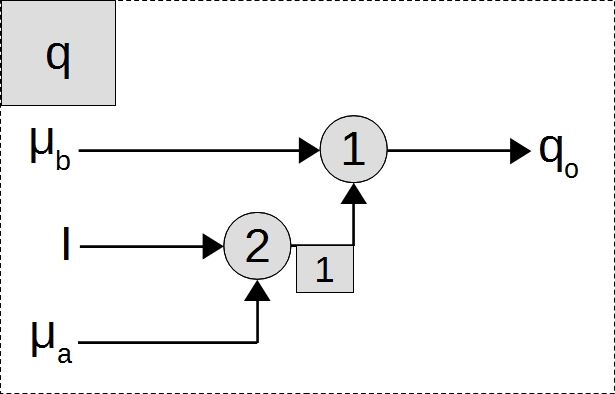
\includegraphics[scale=0.3]{figures/SDFG_q}
  \caption{Synchronous data flow graph of the q block in the guided image filter}
  \label{fig:sdfg_q}
\end{figure}

To find the parallelism in the system precedence graphs (PG) have to be created. Since the subsystems are simple the precedence graphs can be created looking at the system from end to start and for each operator find out which signal is needed and have to be calculated before. Another method is to create a synchronous data flow graph (SDFG) and from the SDFG a matrix, $\uuline\Gamma$, can be created. This matrice expresses the relationship between the in- and outputs from each node in the SDFG and is called the \textit{topology} matrix. An example of an SDFG is illustrated on in figure \ref{fig:sdfg_q}. In this example the topology matrix is then:
\begin{equation}
  \begin{array}{ c c c }
    & & \text{nodes} \\
  \uuline\Gamma = & \text{arcs} & 
  \begin{bmatrix}
   -1 & 1 
  \end{bmatrix}
  \end{array}
\end{equation}
If $rank(\uuline \Gamma) \leq s-1$ where $s$ is the number of nodes then a positive integer vector $\uline q$ can be found such that $\uuline\Gamma \cdot \uline q = \uline 0$. Then resulting $\uline q$ is:
\begin{equation}
  \uline{q} =
  \begin{bmatrix}
  1 \\
  1
  \end{bmatrix}
\end{equation}
This $\uline q$ vector expresses how many times each node have to be executed within one sample period.\\

With $\uuline \Gamma$ and $\uline q$ a periodic admissible sequential sequence (PASS) can be found. This tells a sequential sequence in which the nodes can be executed and with it, a periodic admissible parallel sequence (PAPS) can be generated. To find the PASS generate a randomly ordered list of all the nodes, $L$. For each 

\section{Allocation and Scheduling}
To develop a Finite State Machine (FSM) we need to know which hardware is allocated and when each operation is scheduled. This enables us to define some states for the FSM.

From section~\vref{sec:paraanal} some precedence graphs are found and theses graphs shows how many FUs can run in parallel 

\todo{Skitse. skal skrives om på et tidspunkt} To figure out how much can be allocated to the system we have started a new project in Xilinx Vivado 2016.2, chosen ZEDboard with a Zynq Z-7020 as the target and then generate a block design with a chosen element (adder, multiplier, etc.). TCL commands are used to copy the first element 99 times and connecting the inputs to the same input and generate a separate output for each element. Then let Vivado generate its own VHDL wrapper for the block design and run synthesis. Then look in the project summary for utilization. When Re-customizing the IP blocks the signal width are kept as standard and everything else is set for high speed. \\  
\begin{table}[ht!]
\centering
\begin{tabular}{l | c c c c c }
  \toprule
   &  LUT & LUTRAM & FF & BRAM & DSP48 \\
  \midrule
  Adder & 15 & - & 15 & - & - \\
  Adder/Subtracter  & 16 & - & 15 & - & - \\
  Subtract  & 15 & - & 15 & - & - \\
  Multiplier - LUT  & 352 & - & 36 & - & - \\
  Multiplier - DSP48 & - & - & - & - & 1 \\
  Divider & 680 & 1 & 150 & 0.5 & 8 \\
  \bottomrule
\end{tabular}
\caption{Number of logic elements used in average for each operator}
\label{tab:utilizationofelements}
\end{table}

\newpage
% precedence graphs
\begin{figure}[ht!]
  \centering
  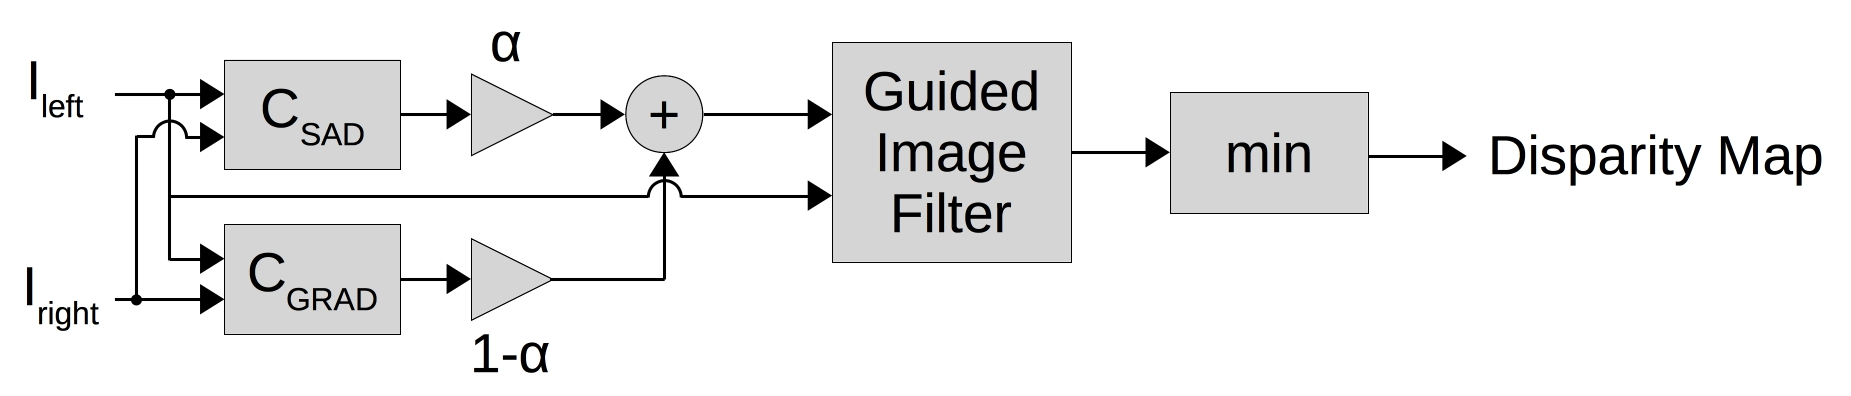
\includegraphics[scale=0.3]{figures/whole_system}
  \caption{Data flow graph of the whole system}
  \label{fig:whole_system}
\end{figure}

\begin{figure}[ht!]
  \centering
  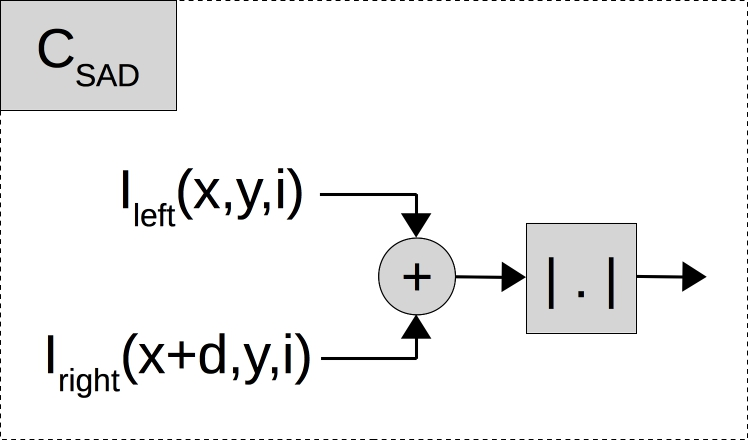
\includegraphics[scale=0.3]{figures/c_sad}
  \caption{Data flow graph of the $C_{SAD}$ block in figure \ref{fig:whole_system}}
  \label{fig:c_sad}
\end{figure}

\begin{figure}[ht!]
  \centering
  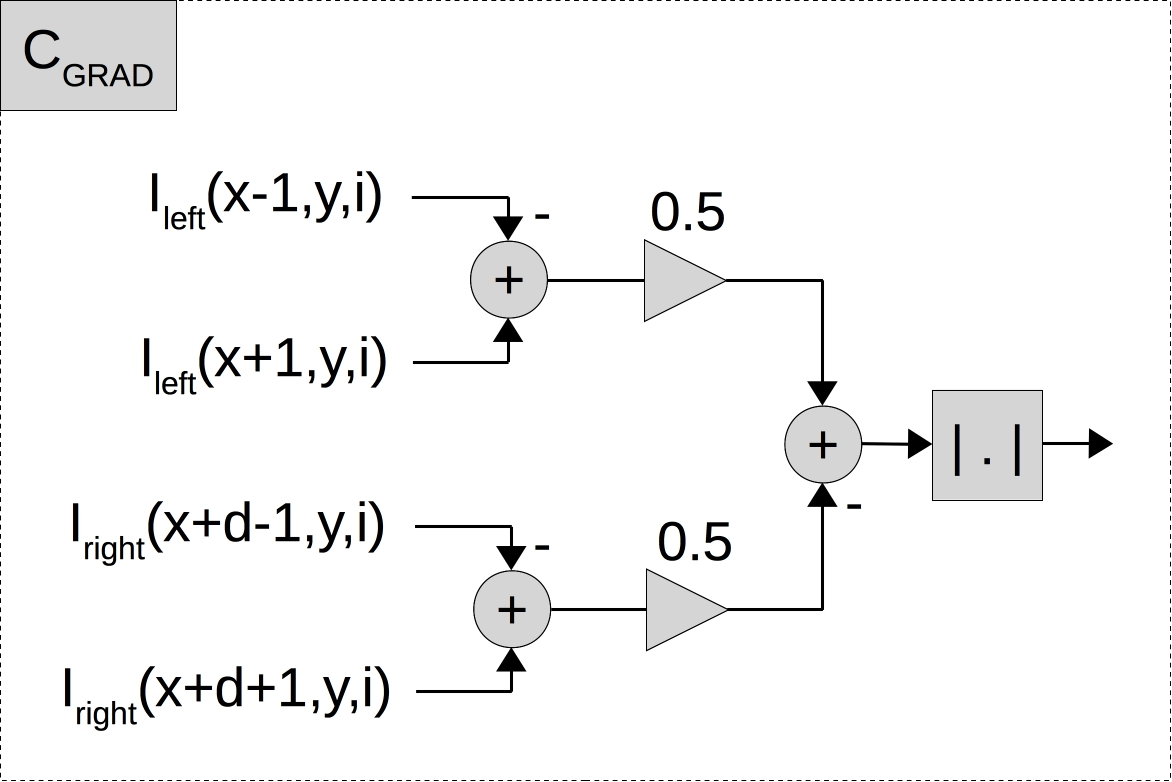
\includegraphics[scale=0.3]{figures/c_grad}
  \caption{$C_{GRAD}$ ikke sikker}
  \label{fig:c_grad}
\end{figure}

\begin{figure}[ht!]
  \centering
  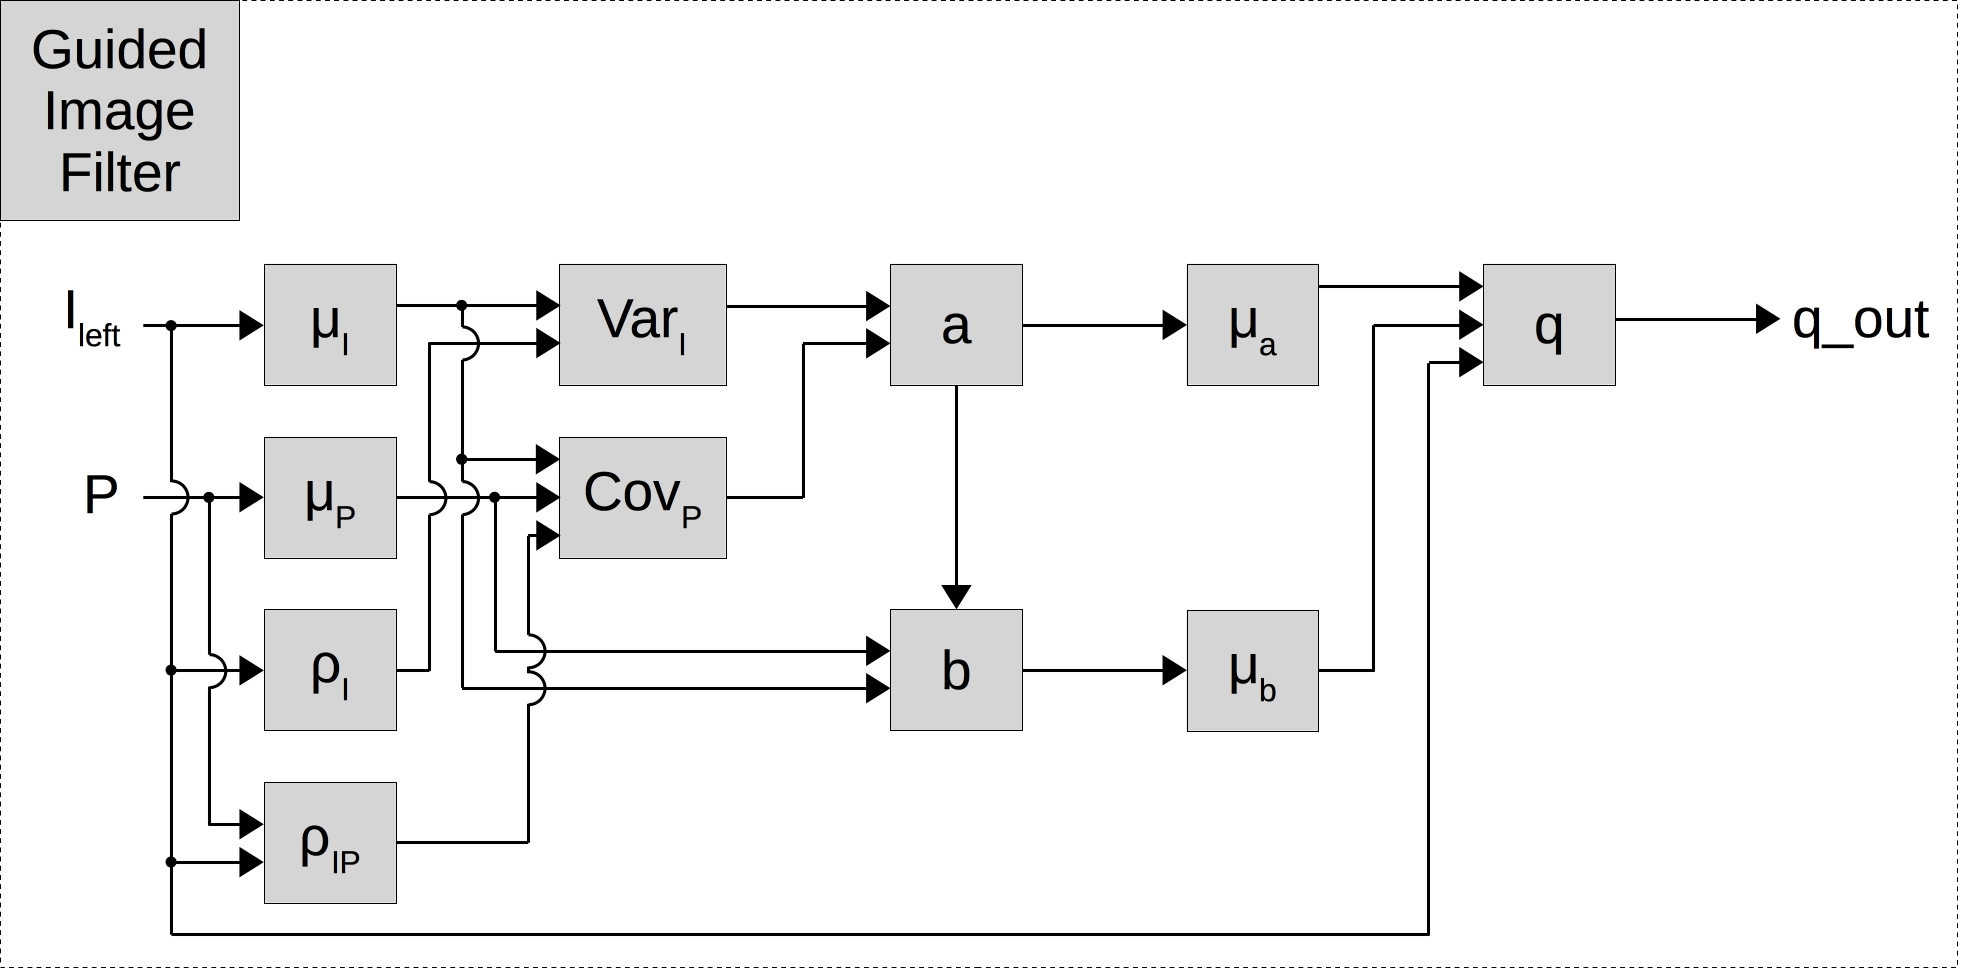
\includegraphics[scale=0.3]{figures/guided_image_filter}
  \caption{Guided image filter}
  \label{fig:Guided_image_filter}
\end{figure}

\begin{figure}[ht!]
  \centering
  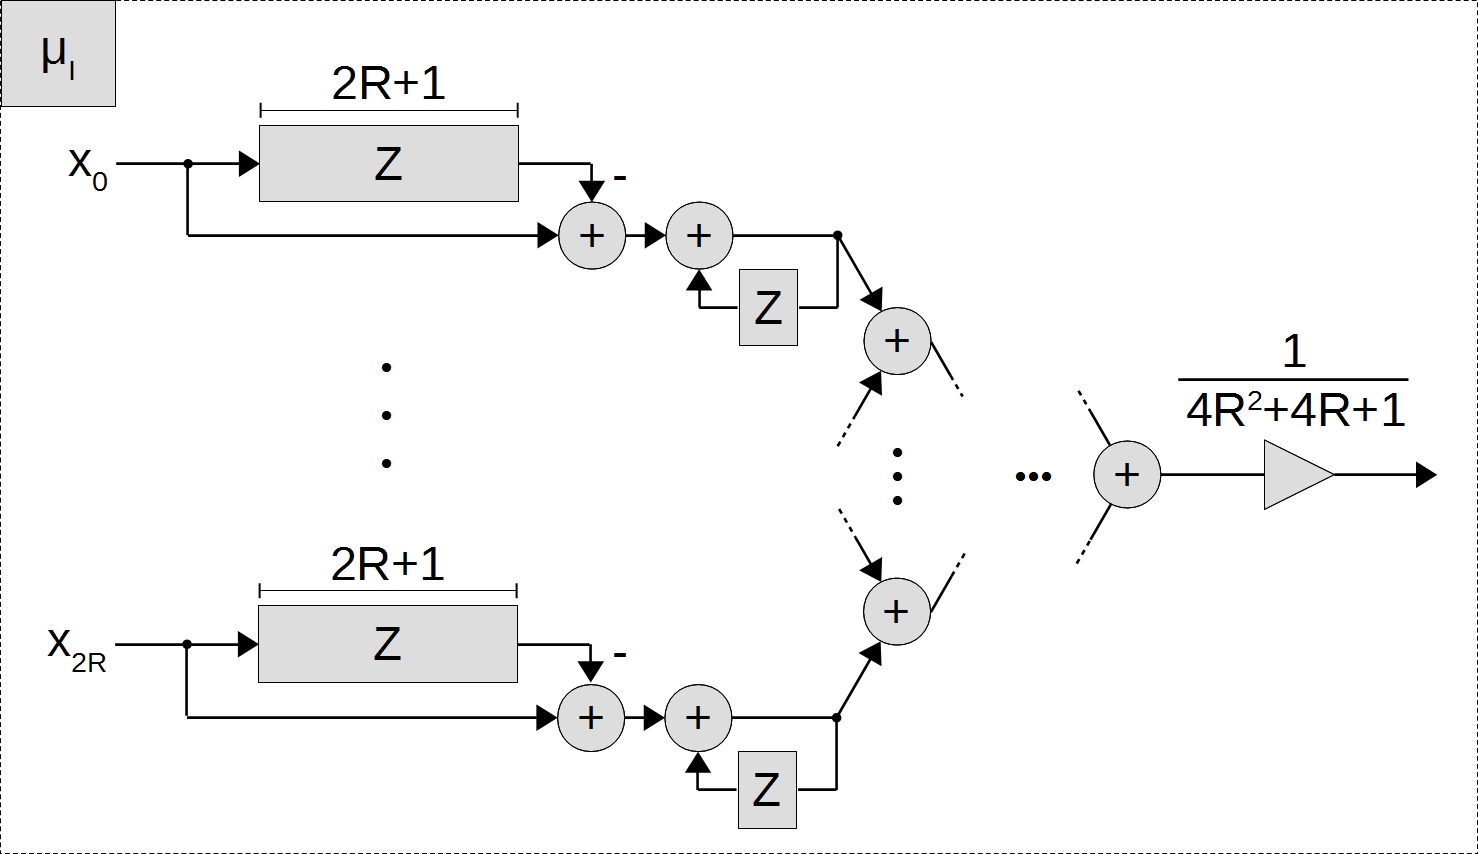
\includegraphics[scale=0.3]{figures/mean}
  \caption{Mean filter}
  \label{fig:mean}
\end{figure}

\begin{figure}[ht!]
  \centering
  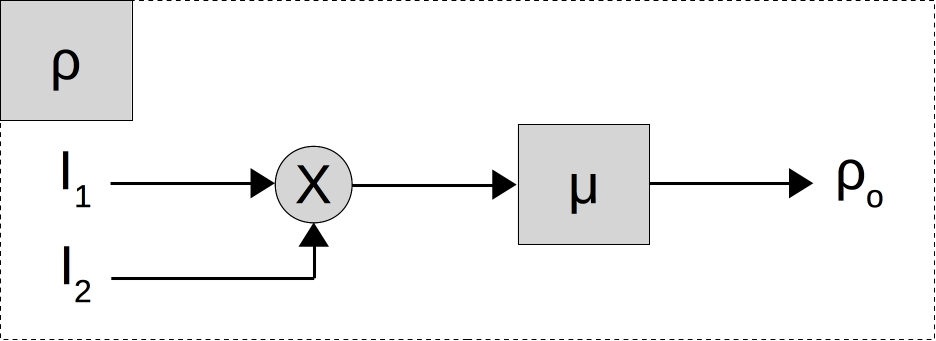
\includegraphics[scale=0.3]{figures/rho}
  \caption{Correlation}
  \label{fig:rho}
\end{figure}

\begin{figure}[ht!]
  \centering
  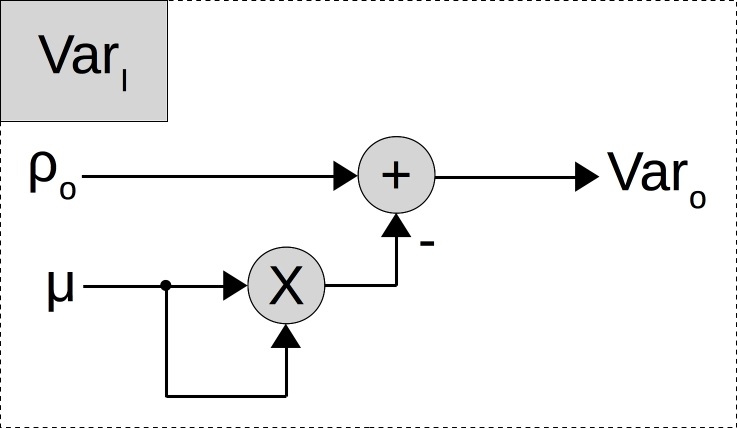
\includegraphics[scale=0.3]{figures/var_par}
  \caption{Variance}
  \label{fig:var_par}
\end{figure}

\begin{figure}[ht!]
  \centering
  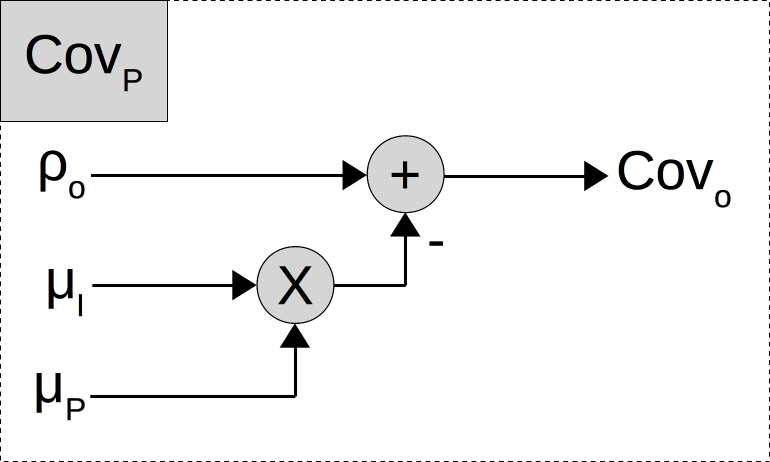
\includegraphics[scale=0.3]{figures/cov_par}
  \caption{Covariance}
  \label{fig:cov_par}
\end{figure}

\begin{figure}[ht!]
  \centering
  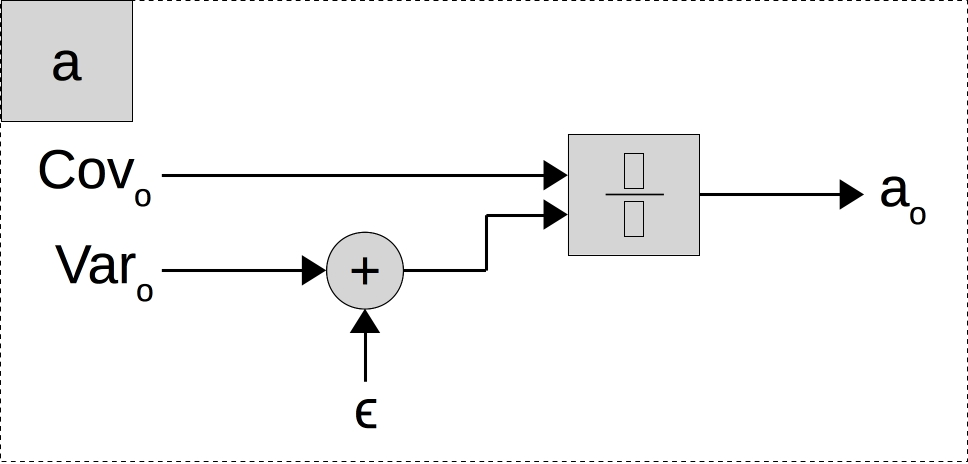
\includegraphics[scale=0.3]{figures/a_par}
  \caption{A box}
  \label{fig:a_par}
\end{figure}

\begin{figure}[ht!]
  \centering
  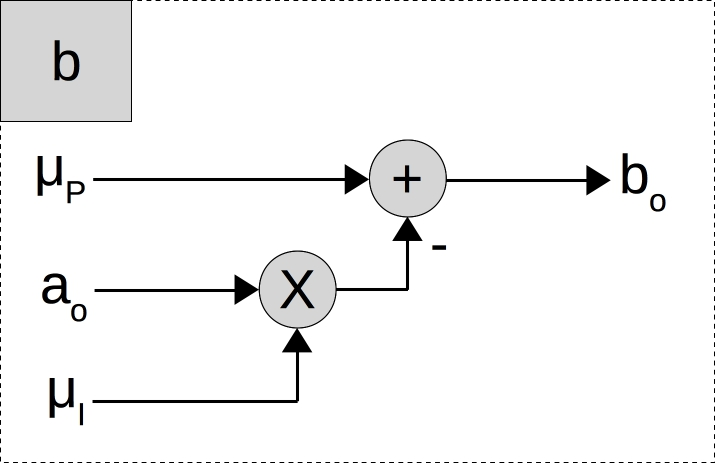
\includegraphics[scale=0.3]{figures/b_par}
  \caption{B box}
  \label{fig:b_par}
\end{figure}

\begin{figure}[ht!]
  \centering
  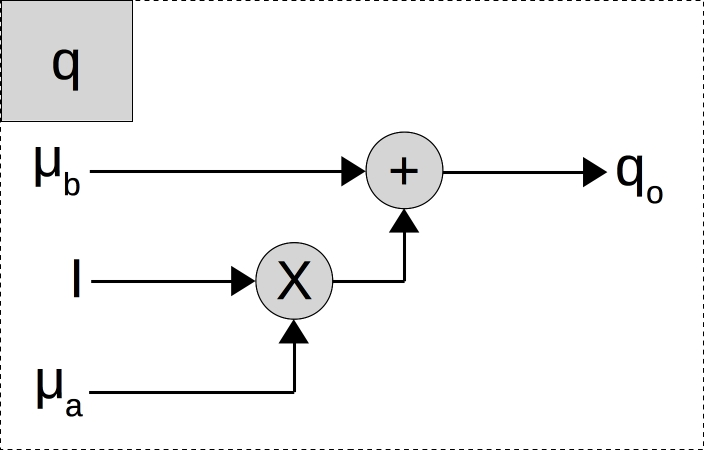
\includegraphics[scale=0.3]{figures/q_par}
  \caption{Q box}
  \label{fig:q_par}
\end{figure}

\color{gray}
\section*{noter til mig selv}
% ---------------------- udkommentere senere --------****
lav dfg -> pg -> architecture. dette er steppet mellem algoritme og arkitektur domænerne i A3 modellen. Se første side i mm7 i reconf. kursuset. \\ 


DSP ALG -> Precedence Graph -> Control data flow graph -> scheduling/allocation -> FSMD specification -> assignment -> architecture\\
mm7 side (3) Force Directed Scheduling\\

% links https://en.wikipedia.org/wiki/Analysis_of_parallel_algorithms
Wanhammer \cite{wanhammer1999} side 244 i pdf / 229 i bogen:\\
Precedence graphs. De beskriver in hvilken rækkefølge forskellige events (a,b,c) sker. order of occurrences of events\\
Latency: dette er tiden tager at genere et output fra man har modtaget input.

Throughput: dette er tiden mellem outputs

Interleaving: increase throughput af sekventielle algoritmer.


~\\
Fra wiki: https://en.wikipedia.org/wiki/Analysis\_of\_parallel\_algorithms\\
tag det med en gran salt. er nok hovedsagligt til General Purpose Processors (GPP)\\
$p$ processors, $T_p$ time computation
\begin{itemize}
 \item \textit{work}: total number of operations on the processors. Is equal to $T_1$.
 \item \textit{span}: the critical path. Length of longest series of data dependent operations. Is equal to $T_\infty$
 \item \textit{cost}: is $pT_p$ and describes the total time spent by all $p$ on both waiting and computing.
\end{itemize}
Laws:
\begin{itemize}
  \item \textit{Work law}: $pT_p \geq T_1$. the cost is at least equal to the work
  \item \textit{Span law}: $T_p \geq T_\infty$. a finite number of processors, $p$, can't outperform an infinite number of processors
\end{itemize}
With these definitions and laws the following measures of performance can be given:
\begin{itemize}
  \item \textit{Speedup}: is the gain in speed when comparing parallel execution to sequential execution: $S_p = T_1 / T_2$
  \item \textit{Efficiency}: is the speedup per processor: $S_p / p$
  \item \textit{Parallelism}: is the ratio $T_1 / T_\infty$ and it describes the maximum speedup on any number of processors. By \textit{span law} the \textit{parallelism} bounds the speedup: if $p>T_1/ T_\infty$ then $T_1/T_p \leq T_1 / T_\infty < p$ 
  \item \textit{Slackness}: is $T_1/(pT_\infty)$. a slackness than one implies (by span law) that perfect linear speedup is impossible on $p$ processors.
\end{itemize}
Execution on a limited number of processors\\
Parallelitets analyse bliver normalt udført under den antagelse at man har et ubegrænset antal processor tilgængeligt. Dette er selvfølgelig ikke realistisk men ikke et problem da hvilken som helst beregning som kan laves på $N$ processorer kan også blive udført på $p$ processorer hvor $p < N$ ved at lade hver processor udføre flere "enheders" arbejde. \\
Brent's law:\\
$T_p \leq T_N + \dfrac{T_1 - T_N}{p}$ \\
$T_p = O \left( T_N + \dfrac{T_1}{p} \right)$\\
$\dfrac{T_1}{p} \leq T_p < \dfrac{T_1}{p} + T_\infty$ det viser at \textit{span} og \textit{work} giver nogle fornuftige grænser for computation time.\\
\color{black}

%\section{Optimization}

\section{FSMD design}

\section{VHDL + Simulation}

%\section*{Box filter / Mean function}
%\todo{this section should contain the design for my boxfilter or mean function}
%As seen from the guided image filter algorithm the mean function $f_{mean}(x)$ is used multiple q
%
%%\subsection*{Finite State Machine}
%\todo{beskriv FSM'en jeg har lavet (se figur 6.1) }
%\begin{figure}
%  \centering
%  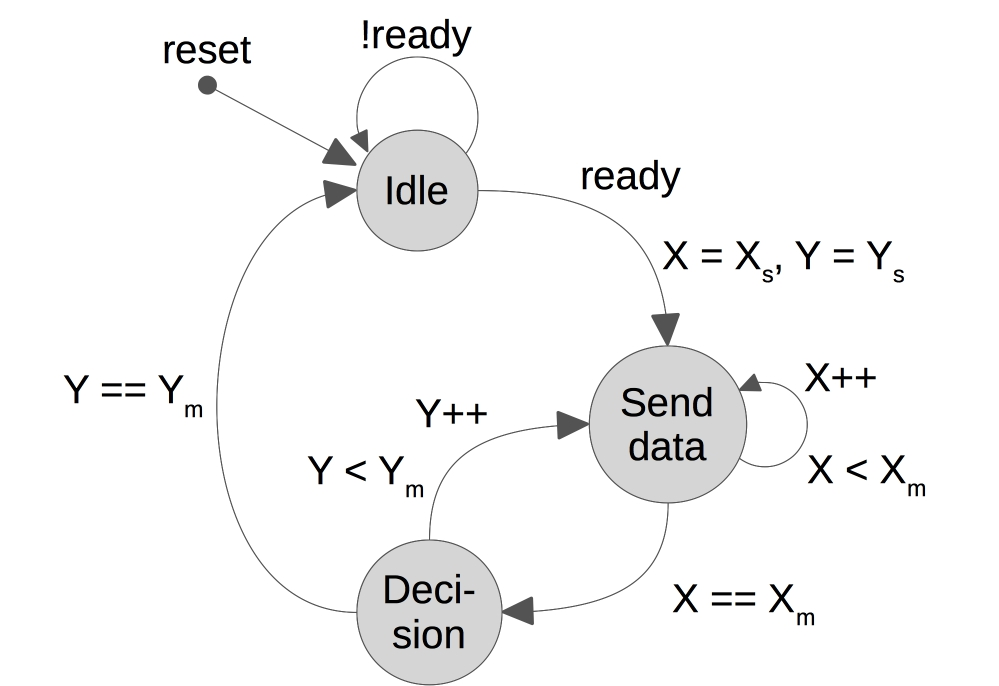
\includegraphics[width=0.5\textwidth]{figures/meanFSMv1.jpg}
%  \caption{TEXT GOES HERE}
%  \label{fig:LABEL}
%\end{figure}
%
%\subsection*{Memory}
%\begin{figure}
%  \centering
%  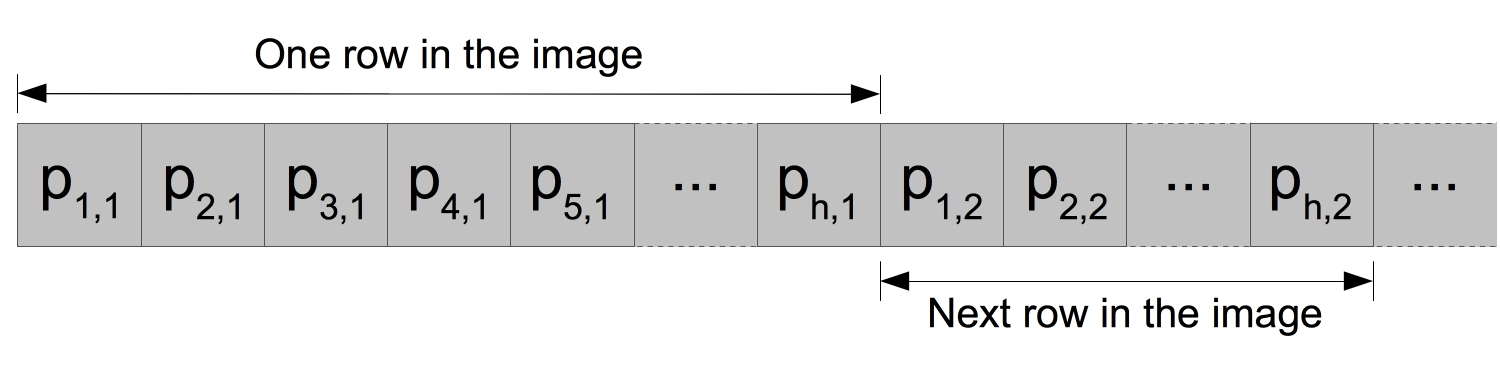
\includegraphics[width=0.5\textwidth]{figures/memdata.jpg}
%  \caption{TEXT GOES HERE}
%  \label{fig:LABEL}
%\end{figure}
%
%memory requirement: \\
%$3 \cdot 8$ bits per pixel (rgb image). test image is $741 \times 497$ so for the test image $8.838.648$ bits $\approx$ 9 megabit $\approx$ 1.1 megabyte.
%
%\subsection*{VHDL/Simulation}
%\todo{skriv om VHDL kode og simulation af filteret}
%
%\subsection*{Implementation/Test}
%\todo{skriv om implementation på FPGA'en og gerne verificere det virker}
%
